\section{Appendix name}

Some appendix text.
\begin{figure}[H] %The [H] flag forces the figure placement to land HERE. (requires float package)
    \centering
    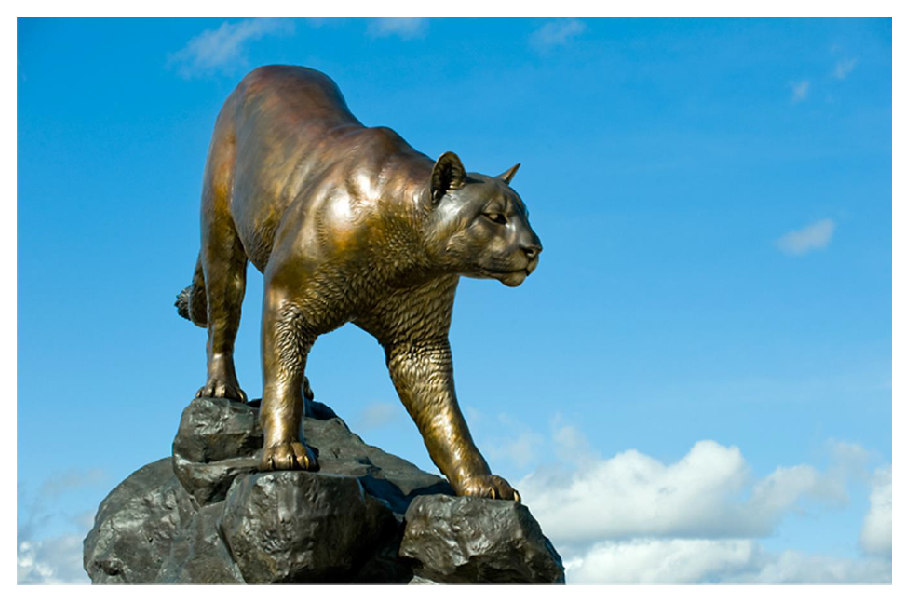
\includegraphics[width=0.4\linewidth]{butch}
    \caption{An image of the Butch statue taken from the 2015-2016 Graduate Student Survival Guide.}
    \label{fig:a1}
\end{figure}
And this is an equation in the appendix
\begin{align}
    F=ma,
\end{align}  
and this is a table
\begin{table}[H]
\centering
\begin{tabular}{|c||c|c|}
  \hline
  % after \\: \hline or \cline{col1-col2} \cline{col3-col4} ...
  a  & 1 & 2 \\\hline
  b  & 3 & 4 \\
  c  & 5 & 6 \\
  \hline
\end{tabular}
\caption{A table}
\end{table}